\section{第二问的敏感性与模型边界}
\label{q2-limits}

\subsection{交换系数对不同输出的影响}
为比较边界参数的作用，在相同$N=320$网格上分别将$h_m$和$h_T$
降低、提高20\%，其余条件保持不变并联立求解。
对$p\in\{h_m,h_T\}$，定义含水率的归一化中心割线
\begin{equation}
 E_{C,p}^{(20\%)}(t,r)=
 \frac{C_{1.2p}(t,r)-C_{0.8p}(t,r)}{0.4C_p(t,r)}.
\label{q2-eq-sensitivity}
\end{equation}
分母采用同网格的未扰动解，而非不同精度等级的正式外推场。
这是给定扰动范围的确定性灵敏度，不是精确微分导数、实验置信区间或参数最优值。

\begin{figure}[htbp]
\centering
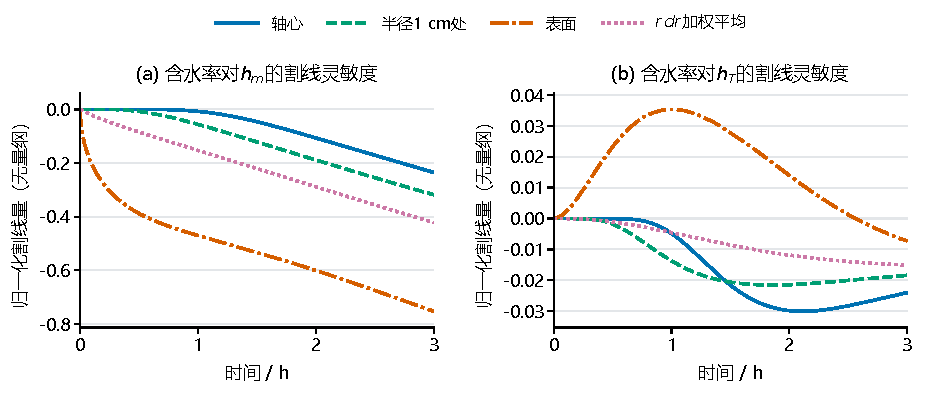
\includegraphics[width=\textwidth]{figures/q2_sensitivity.pdf}
\caption{前3\unit{h}含水率对交换系数的割线灵敏度：左为$h_m$，右为$h_T$；各曲线对应轴心、半径1\unit{cm}、表面和$r\,\mathrm dr$加权平均。}
\label{q2-fig-sensitivity}
\end{figure}

\begin{table}[htbp]
\centering\small
\caption{3\unit{h}含水率的归一化割线灵敏度}
\label{q2-tab-sensitivity}
\begin{tabular}{@{}lrr@{}}
\toprule
位置或平均量 & $E_{C,h_m}^{(20\%)}$ & $E_{C,h_T}^{(20\%)}$\\
\midrule
轴心 & $-0.235100$ & $-0.023994$\\
半径1\unit{cm} & $-0.318258$ & $-0.018379$\\
表面 & $-0.753442$ & $-0.007208$\\
$r\,\mathrm dr$加权平均 & $-0.421969$ & $-0.015038$\\
\bottomrule
\end{tabular}
\end{table}

表\ref{q2-tab-sensitivity}显示，在$3\unit{h}$含水率这一输出上，
$h_m$的相对扰动影响更大，且表面最敏感；提高$h_m$使失水加快。
这不表示换热系数在整个时域不重要：$h_T$的$\pm20\%$情景在前
$3\unit{h}$可使表面温度与同网格基线最多相差1.0981\unit{K}。
因此“主导参数”必须同时指定输出、位置、时刻及扰动范围。
改用PCHIP环境插值时，全场最大温差约0.005715\unit{K}、
含水率差约$1.65\times10^{-5}\unit{kg/kg}$，也说明输入重构的不确定性
与数值离散误差应分别讨论。

\subsection{等效水分边界的含义与可识别性}
一般的表面平衡量应写成$b=g(y_\infty,T_s,\ldots)$。
在固定均匀环境、$D>0$和$h_m>0$时，本模型的平衡状态为$C=b$：
$h_m$主要影响接近平衡的速率，映射$g$则决定平衡位置。
文献通过平衡干基含水率或解吸等温线连接材料与气相\cite{dasilva2014,adrover2020}，
为区分这两个角色提供依据，但不提供本药材的映射参数。

现有数据只给外部驱动，缺少样品温度、含水率和失重响应，
不能用模型自身预测重新标定$g$和$h_m$。
即使知道某条表面轨迹和归一化通量$\hat q$，允许自由时间映射时，
不同$h_m^*>0$仍可用$b^*=C_s-\hat q/h_m^*$产生相同通量；
在满足$b^*\geq0$等物理约束的子集中仍可能非唯一。
因此，应先确认环境水分的质量基准，再补充本药材解吸关系、干质量及配套的
失重和温度响应，才能检验受限参数族的可识别性。

式\eqref{q2-eq-boundary}中的$h_m(C_s-b)$尚不是
$\mathrm{kg/(m^2\cdot s)}$的真实质量通量。
若改用气相浓度差$j_s=k_g(c_{v,s}-c_{v,\infty})$，即使$k_g$同样以m/s计，
也不能直接沿用$h_m$的数值；只有在线性化映射
$c_{v,s}-c_{v,\infty}=K(C_s-b)$及一致干密度口径下，才有
$\rho_{d,\mathrm{ref}}h_m=k_gK$。目前保留恒等映射作为明确假设，
不据局部小扰动灵敏度较弱便宣称真实映射误差很小。

\subsection{组成守恒与相变扩展的必要条件}
若将附录3的$\rho(C)$视为真实湿体密度，则
\begin{equation}
 \rho_d(C)=\frac{650+128C}{1+C},\qquad
 \rho_d'(C)=-\frac{522}{(1+C)^2}.
\label{q2-eq-density}
\end{equation}
静止固定骨架应满足$\partial_t\rho_d=0$，
但式\eqref{q2-eq-density}在失水时会使干密度增加。
所以不能同时将固定体积、无干物质生成和该真实变密度解释作为精确关系。
本文采用有效容量$S(C)$，严格组成守恒的升级则需要相容的密度、孔隙和几何闭合。

潜热也不能作为与质量模型无关的单独修正。以固定骨架和常压参考为例，
设每kg干物质焓为$\mathcal H(T,C)$，偏水焓为
$\overline h_w=\partial_C\mathcal H$，在忽略机械功且内部无相变时，
一组相容的质量--能量表达为
\begin{equation}
 \rho_d C_t+\nabla\cdot\boldsymbol j_w=0,\qquad
 \partial_t(\rho_d\mathcal H)
 +\nabla\cdot(\boldsymbol q+\overline h_w\boldsymbol j_w)=0,
 \quad\boldsymbol q=-k\nabla T.
\label{q2-eq-enthalpy}
\end{equation}
用质量式消去组成储存项后，温度形式为
\begin{equation}
 \rho_d\mathcal H_T T_t=
 \nabla\cdot(k\nabla T)-\boldsymbol j_w\cdot\nabla\overline h_w.
\label{q2-eq-enthalpy-reduced}
\end{equation}
这说明组成焓、携焓通量和储存项需联合定义，不能只将左侧改为
$\partial_t[S(C)(T-T_{\mathrm{ref}})]$便称更守恒。
表面若有向外蒸发通量$j_s$，还应以相同通量闭合气固平衡和能量：
\begin{equation}
 q_n=h_T(T_s-T_\infty)+q_{\mathrm{rad,out}}
       +[h_v(T_s)-\overline h_w(T_s,C_s)]j_s.
\label{q2-eq-surface-enthalpy}
\end{equation}
水蒸气焓与偏水焓必须使用同一水的参考态，才能使其差与能量零点选择无关。
表面蒸发与域内相变、扩散携焓是不同机制\cite{comsol}；
局部$C_t$包含相邻区域的水分交换，不能直接冒充内部蒸发率。

题目未给解吸或水活度关系、组成焓和实际质量交换数据，故上述方程仅说明
物理扩展所需闭合，不用于替换当前数值答案。
同样，辐射还需壁温、视角和发射率，收缩还需材料运动与干物质守恒，
本问没有凭无来源参数填补这些机制。离散精度检验支持给定方程的数值可靠性，
并不证明这些省略机制足够小或真实预测具有四位精度。

\subsection{输出时域与后续问题的衔接}
第二问要求整个烘干过程的模型，论文表明确展示前$3\unit{h}$，
而逐秒Excel没有另行写明结束时刻。本文将$1$至$10800\unit{s}$作为
该文件的工作性时域解释，完整给出这一时段的规定径向采样，
不将其称为已经计算至真实干燥结束。
方程形式可继续用于预热之后的阶段，但附件1仅覆盖前$4\unit{h}$；
进一步求终点必须说明环境延拓、停止条件和长期数值验证。
第三问的全域$0.15\unit{kg/kg}$阈值将单独处理，
不以背景中的2--3天替代结束条件，也不把前$3\unit{h}$的几何或精度结论
直接外推到低含水率的长期过程。
\FloatBarrier
